\documentclass{article}

\usepackage{fancyhdr}
\usepackage{extramarks}
\usepackage{amsmath}
\usepackage{amsthm}
\usepackage{amsfonts}
\usepackage{tikz}
\usepackage[plain]{algorithm}
\usepackage{algpseudocode}
\usepackage{graphicx}
\usetikzlibrary{automata,positioning}
\usepackage{pdfpages}

%
% Basic Document Settings
%

\topmargin=-0.45in
\evensidemargin=0in
\oddsidemargin=0in
\textwidth=6.5in
\textheight=9.0in
\headsep=0.25in

\linespread{1.1}

\pagestyle{fancy}
\lhead{\hmwkAuthorName}
\chead{\hmwkClass\ (\hmwkClassInstructor\ \hmwkClassTime): \hmwkTitle}
\rhead{\firstxmark}
\lfoot{\lastxmark}
\cfoot{\thepage}

\renewcommand\headrulewidth{0.4pt}
\renewcommand\footrulewidth{0.4pt}

\setlength\parindent{0pt}

%
% Create Problem Sections
%

\newcommand{\enterProblemHeader}[1]{
    \nobreak\extramarks{}{Problem \arabic{#1} continued on next page\ldots}\nobreak{}
    \nobreak\extramarks{Problem \arabic{#1} (continued)}{Problem \arabic{#1} continued on next page\ldots}\nobreak{}
}

\newcommand{\exitProblemHeader}[1]{
    \nobreak\extramarks{Problem \arabic{#1} (continued)}{Problem \arabic{#1} continued on next page\ldots}\nobreak{}
    \stepcounter{#1}
    \nobreak\extramarks{Problem \arabic{#1}}{}\nobreak{}
}

\setcounter{secnumdepth}{0}
\newcounter{partCounter}
\newcounter{homeworkProblemCounter}
\setcounter{homeworkProblemCounter}{1}
\nobreak\extramarks{Problem \arabic{homeworkProblemCounter}}{}\nobreak{}

%
% Homework Problem Environment
%
% This environment takes an optional argument. When given, it will adjust the
% problem counter. This is useful for when the problems given for your
% assignment aren't sequential. See the last 3 problems of this template for an
% example.
%
\newenvironment{homeworkProblem}[1][-1]{
    \ifnum#1>0
        \setcounter{homeworkProblemCounter}{#1}
    \fi
    \section{Problem \arabic{homeworkProblemCounter}}
    \setcounter{partCounter}{1}
    \enterProblemHeader{homeworkProblemCounter}
}{
    \exitProblemHeader{homeworkProblemCounter}
}

%
% Homework Details
%   - Title
%   - Due date
%   - Class
%   - Section/Time
%   - Instructor
%   - Author
%

\newcommand{\hmwkTitle}{Homework\ \#5}
\newcommand{\hmwkDueDate}{October 20, 2019}
\newcommand{\hmwkClass}{CMSE 820}
\newcommand{\hmwkClassTime}{}
\newcommand{\hmwkClassInstructor}{Professor Yuying Xie}
\newcommand{\hmwkAuthorName}{\textbf{Boyao Zhu}}

%
% Title Page
%

\title{
    \vspace{2in}
    \textmd{\textbf{\hmwkClass:\ \hmwkTitle}}\\
    \normalsize\vspace{0.1in}\small{Due\ on\ \hmwkDueDate\ at 11:59pm}\\
    \vspace{0.1in}\large{\textit{\hmwkClassInstructor\ \hmwkClassTime}}
    \vspace{3in}
}

\author{\hmwkAuthorName}
\date{}

\renewcommand{\part}[1]{\textbf{\large Part \Alph{partCounter}}\stepcounter{partCounter}\\}

%
% Various Helper Commands
%

% Useful for algorithms
\newcommand{\alg}[1]{\textsc{\bfseries \footnotesize #1}}

% For derivatives
\newcommand{\deriv}[1]{\frac{\mathrm{d}}{\mathrm{d}x} (#1)}

% For partial derivatives
\newcommand{\pderiv}[2]{\frac{\partial}{\partial #1} (#2)}

% Integral dx
\newcommand{\dx}{\mathrm{d}x}

% Alias for the Solution section header
\newcommand{\solution}{\textbf{\large Solution}}

% Probability commands: Expectation, Variance, Covariance, Bias
\newcommand{\E}{\mathrm{E}}
\newcommand{\Var}{\mathrm{Var}}
\newcommand{\Cov}{\mathrm{Cov}}
\newcommand{\Bias}{\mathrm{Bias}}

\begin{document}

\maketitle

\pagebreak

\begin{homeworkProblem}
\textbf{Solution}\\
\textbf{a.}\\
The \(l_{2,1}\) norm 
\[
f(X) = \lVert X\rVert_{2,1} = \Sigma_j\lVert X_{.,j}\rVert_2 = \Sigma_j\sqrt{\Sigma_i X^2_{ij}}
\]
To show that \(f(X)\) is a convex function X, one needs to show that \(f(X)\) is a norm of \(X\), as convexity follows directly from the definition of norms.
\begin{itemize}
    \item By construction, it's clear that for any matrix \(X, f(X)\geq0\).
    \item 
    \[
    f(X) = 0 \Leftrightarrow \Sigma_j\sqrt{\Sigma_i X^2_{ij}} = 0 \Leftrightarrow \forall i, j, X_{ij}=0 \Leftrightarrow X = 0
    \]
    \item \(\forall \alpha\in\mathbb{R}\)
    \[
    f(\alpha X) = \Sigma_j\sqrt{\Sigma_i(\alpha X_{ij})^2}= \lvert x\rvert \Sigma_j\sqrt{\Sigma_i X_{ij}^2}=\lvert\alpha\rvert f(X)
    \]
    \item \(\forall X, Y\)
    \[
    f(X+Y) = \Sigma_j\lVert(X+Y)_{.,j}\rVert_2 \leq\Sigma_j(\lVert X_{.,j}\rVert_2+\lVert Y_{.,j}\rVert_2) = \Sigma_j\lVert X_{.,j}\rVert_2+\Sigma_j\lVert Y_{.,j}\rVert_2 = f(X)+f(Y).
    \]
Note that the inequality follows from the triangle inequality for the \(l_2\) norm of vectors.
    
\end{itemize}

\textbf{b.}\\
\begin{itemize}
	\item If \(X_{.,j}\neq\textbf{0}, f(X)\) is differentiable and convex, so
	\[
	(\partial\lVert X\rVert_{2,1})_{ij} = \frac{\partial f(X)}{\partial X_{ij}} = \frac{X_{ij}}{\lVert X_{.,j}\rVert_2}
	\]
	\item If \(X_{.,j}=\textbf{0}, \text{and} \forall Y\) such that only the \(j\)-th column \(Y_{.,j}\) differs from \(X_{.,j}\).
	\[
	f(Y)-f(X) = \lVert Y_{.,j}\rVert_2
	\]
\end{itemize}
Therefore, 
\[
(\partial \lVert X\rVert_{2,1})_{ij}(X_{.,j}=\textbf{0}) = \{W_{ij}: \lVert W_{.,j}\rVert_2\leq1\}
\]

\textbf{c.}\\
The optimization problem 
\[
\underset{A}{\text{min}}\frac{1}{2}\lVert X-A\rVert_F^2 + \tau\lVert A\rVert_{2,1}
\]
The corresponding Lagragian function \(\mathcal{L}(A)=\frac{1}{2}\lVert X-A\rVert_F^2+\tau\lVert A\rVert_{2,1}\) with subgradient:
\[
(\partial \mathcal{L})_{.,j} = -(X_{.,j}-A_{.,j})+\begin{cases}
									\tau\frac{A_{.,j}}{\lVert A_{.,j}\rVert_2}, \qquad A_{.,j}\neq \textbf{0}\\
									\tau W_{.,j} : \lVert W_{.,j}\rVert_2\leq 1, \qquad A_{.,j}=\textbf{0}
								   \end{cases}
\]
\begin{itemize}
    \item If \(\lVert X_{.,j}\rVert_2\geq\tau\), let \(A_{.,j}=(1-\frac{\tau}{\lVert X_{.,j}\rVert_2})X_{.,j}\), we can verify that 
    \[
      (\partial\mathcal{L})_{.,j}= -(X_{.,j}-(1-\frac{\tau}{\lVert X_{.,j}\rVert_2})X_{.,j})+\tau\frac{X_{.,j}}{\lVert X_{.,j}\rVert_2}=\textbf{0}
    \]
    \item If \(\lVert X_{.,j}\rVert_2 \leq \tau\), let \(A_{.,j}=\textbf{0}\) and choose \(W_{.,j} = X_{.,j}/\tau (\lVert W_{.,j}\rVert_2\leq 1\)), then
    \[
    (\partial \mathcal{L}_{.,j} = -(X_{.,j}) + \tau\frac{X_{.,j}}{\tau}=\textbf{0}
    \]
    Since \(\lVert \cdot\lVert_F^2\) is strictly convex (note the power 2 in the subscript), the optimization problem is also strictly convex.  The unique optimal solution is then given by 
    \[
    A = X\mathcal{S}_{\tau}(\text{diag}(\textbf{x}))\text{diag}(\textbf{x})^{-1}
    \]
where \(x_j = \lVert X_{.,j}\rVert_2\) and the \(j\)-th entry of diag(\(\textbf{x})^{-1}\) is zero if \(x_j=0\).

\end{itemize}

\end{homeworkProblem}


\begin{homeworkProblem}
\textbf{Solution}\\
\textbf{a.}\\
Consider some arbitrary \(x, y\) and \(t\in [0,1].\)  By the definition of \(f(x)\), there exist \(a, b, c(t)\in S\) such that
\[
f(x) = f_a(x), \quad f(y)+f_b(y), \quad f[tx+(1-t)y] = f_{c(t)}[tx+(1-t)y]
\]
Since \(f_c(t)\) are convex, we have
\[
f[tx+(1-t)y] = f_{c(t)}[tx+(1-t)y]\leq tf_{c(t)}(x)+(1-t)f_{c(t)}(y)\leq tf_a(x)+(1-t)f_b(y)=tf(x)+(1-t)f(y)
\]
Hence, \(f(x)\) is convex.\\

\textbf{b.}\\
Let's consider the following general minimization problem:
\[
\begin{split}
\underset{x}{\text{min}} \quad &f(x)\\
\text{subject to} \quad &h_i(x)\leq 0, i = 1, \cdot\cdot\cdot, m,\\
&l_j(x)=0, j = 1, \cdot\cdot\cdot, n.
\end{split}
\]
The corresponding Lagrangian reads
\[
L(x,v,u) = f(x) + v^Th(x) + u^Tl(x), \quad v\in\mathbb{R}^m, u\in\mathbb{R}^n
\]
The dual function is 
\[
g(u,v) = \underset{x}{\text{min}}L(x,u,v)
\]
Now consider some arbitrary \(u_1,u_2\in \mathbb{R}^m, v_1,v_2\in\mathbb{R}^n \text{ and } t\in[0,1]\), we have
\[
\begin{split}
g[tu_1+(1-t)u_2,tv_1+(1-t)v_2] &=\underset{x}{\text{min}}\{f(x)+t[u_1^Th(x) + v_1^Tl(x)]+(1-t)[u_2^Th(x)+v_2^Tl(x)]\}\\
&\geq t\underset{x}{\text{min}}[f(x) + u_1^Th(x)+v_1^Tl(x)]+(1-t)\underset{x}{\text{min}}[f(x)+u_2^Th(x)+v_2^Tl(x)]\\
&= tg(u_1,v_1) + (1-t)g(u_2,v_2)
\end{split}
\]
which shows that the dual function \(g(u,v)\) is concave.\\
The constraint \(u\geq 0\) simply adds a linear term to the Lagrangian, which is both concave and convex.  The dual problem
\[
\underset{u\geq0,v}{max}g(u,v) = -\underset{u\geq0,v}{min}-g(u,v)
\]
is thus a convex optimization problem.

\end{homeworkProblem}

\begin{homeworkProblem}
The Lagrangian for the primal problem reads
\[
L(x,u,v) = \frac{1}{2}x^TQx+c^Tx-u^Tx+v^T(Ax-b)
\]
Note that \(L(x,u,v)\) is a strictly convex function of \(x\), because the quadratic term is strictly convex and the affine terms are convex.  Thus, \(\underset{x}{\text{min }}L(x,u,v)\) has a unique solution \(x^{\ast}\) satisfying \(\frac{\partial L}{\partial x}\lvert_{x=x^\ast}=0\)
\[
\frac{\partial L}{\partial x}\Big |_{x=x^\ast}= Qx^\ast+c-u+A^Tv=0\Leftrightarrow x^\ast=-Q^{-1}(c-u+A^Tv)
\]
Note also that since \(Q\) is positive definite, Ker{\(Q\)}={0}, from which its invertibility follows.\\
The dual problem is 
\[
\underset{u\geq0,v}{\text{max }} g(u,v) + \underset{u\geq0,v}{\text{max }}L(x^\ast,u,v) = \underset{u\geq0,v}{\text{max }}-\frac{1}{2}(c-u+A^Tv)^TQ^{-1}(c-u+A^Tv)+v^Tb.
\]

\end{homeworkProblem}


\begin{homeworkProblem}
I attached coding in the back.  But the program is very slow so that I cannot get the results on time before submitting.  I will upload final results when my program is done.
\end{homeworkProblem}

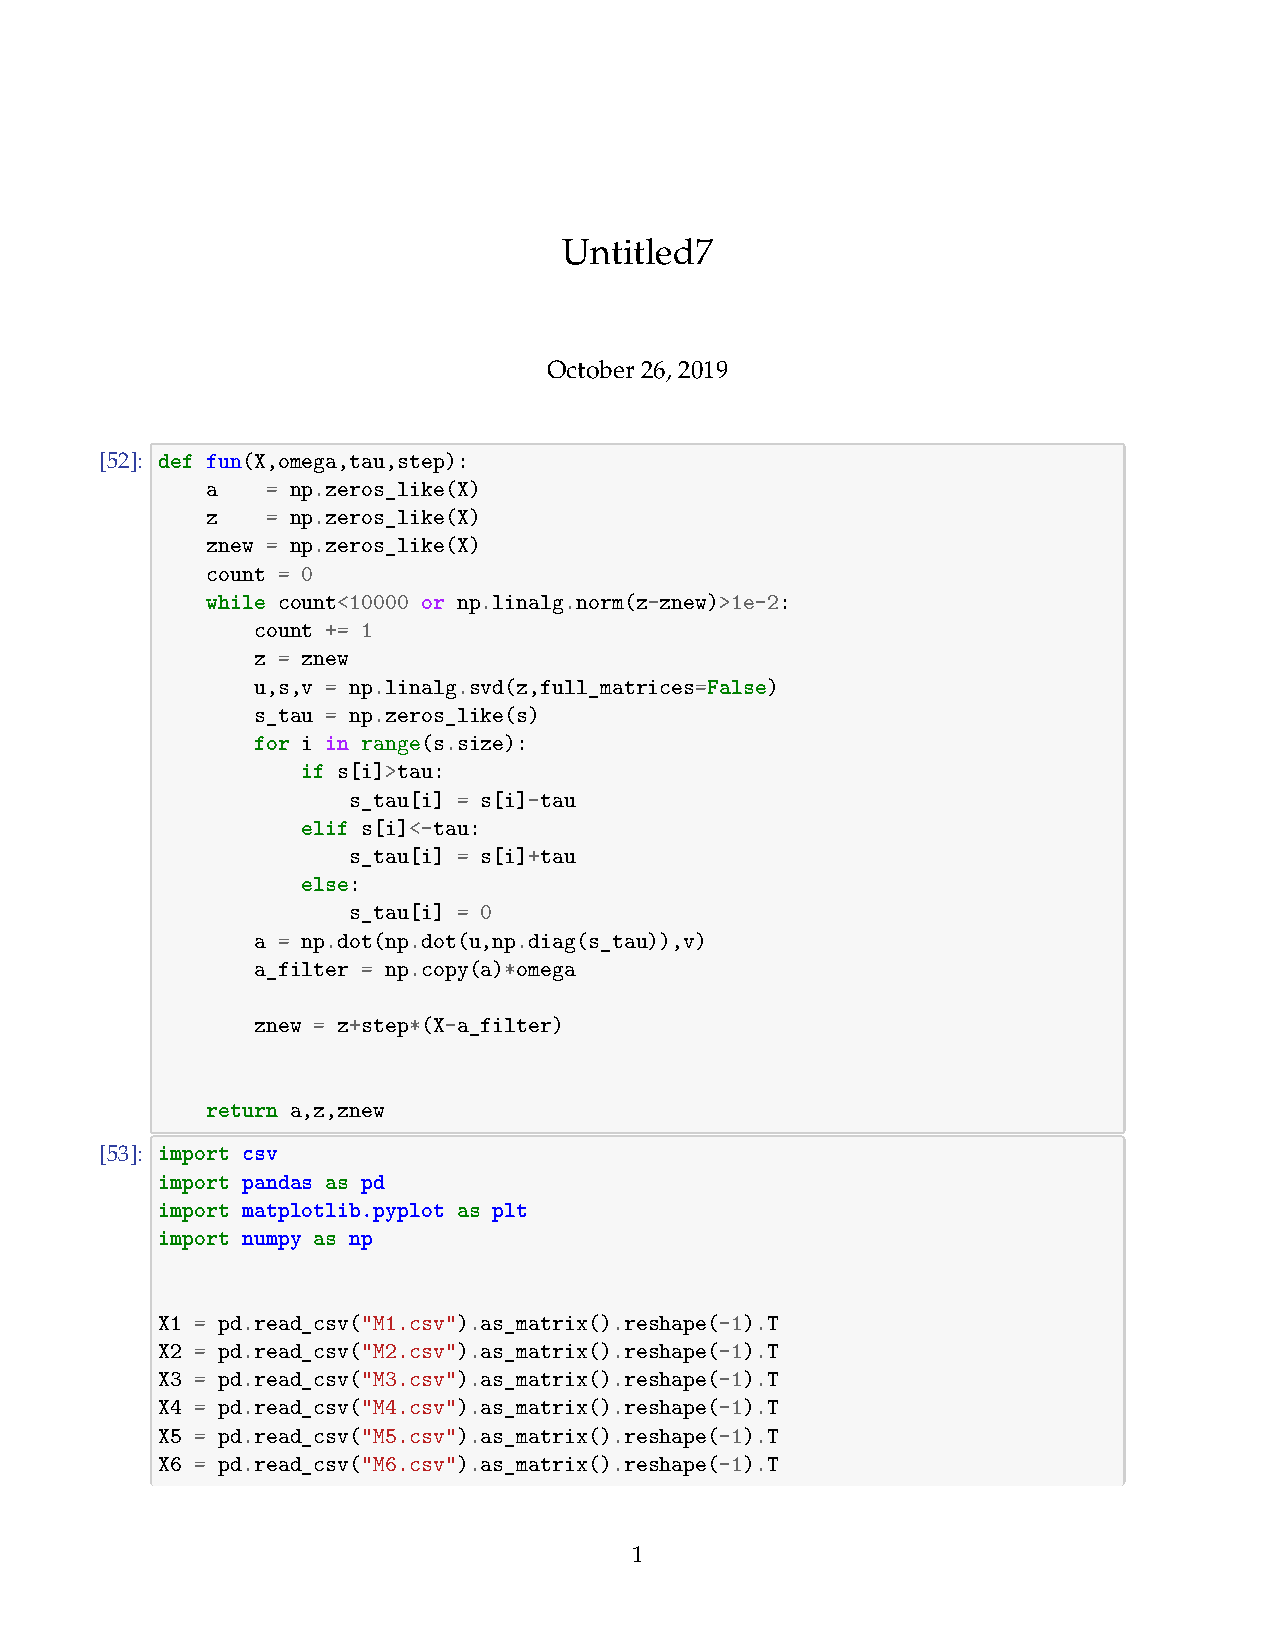
\includepdf[page={-}]{Untitled7.pdf}



























\end{document}